\documentclass[12pt]{elsarticle}
\usepackage{natbib,amsmath}
\special{papersize=8.5in,11in}

\begin{document}


\def\nhdlls{154}
\def\nsource{403265}  % Without UVpSM4, UVES
\def\nspectra{433910}  % Without UVpSM4, UVES
\def\npair{179}  % Within 10"
\def\nlee{several thousands}
\def\hub{h_{72}^{-1}}
\def\umfp{{\hub \, \rm Mpc}}
\def\mew{W_\lambda}
\def\ew{$\mew$}
\def\mzq{z_q}
\def\mfmin{f_{\rm min}}
\def\fmin{$\mfmin$}
\def\zabs{$z_{\rm abs}$}
\def\mzabs{z_{\rm abs}}
\def\msna{{\rm S/N}^{\rm A}_{912}}
\def\sna{S/N$^{\rm A}_{912}$}
\def\mnull{\nu_{\rm 912}}
\def\nnull{$\nu_{\rm 912}$}
\def\intl{\int\limits}
\def\nstatqso{193}
\def\maxoff{0.4}
\def\clls{1.9 \pm 0.2}
\def\alls{5.2 \pm 1.5}
\def\blls{-0.9^{+0.4}_{-0.05}}
\def\cmma{\;\;\; ,}
\def\perd{\;\;\; .}
\def\ltk{\left [ \,}
\def\ltp{\left ( \,}
\def\ltb{\left \{ \,}
\def\rtk{\, \right  ] }
\def\rtp{\, \right  ) }
\def\rtb{\, \right \} }
\def\sci#1{{\; \times \; 10^{#1}}}
\def \rAA {\rm \AA}
\def \mzem {z_{\rm em}}
\def\smm{\sum\limits}
\def \cmm  {cm$^{-2}$}
\def \cmmm {cm$^{-3}$}
\def \kms  {km~s$^{-1}$}
\def \mkms  {{\rm km~s^{-1}}}
\def \lyaf {Ly$\alpha$ forest}
\def \Lya  {Ly$\alpha$}
\def \lya  {Ly$\alpha$}
\def \mlya  {Ly\alpha}
\def \Lyb  {Ly$\beta$}
\def \nhi  {$N_{\rm HI}$}
\def \mnhi  {N_{\rm HI}}
%\def \mtotnhi  {\mnhi^{\rm TOT}}
%\def \totnhi  {$\mtotnhi$}
\def \lnhi {$\log N_{HI}$}
\def \mlnhi {\log N_{HI}}
\def \etal {\textit{et al.}}
\def \ob {$\Omega_b$}
\def \obh {$\Omega_bh^{-2}$}
\def \om {$\Omega_m$}
\def \ol {$\Omega_{\Lambda}$}
\def \gz {$g(z)$}
\def \mgz {g(z)}
\def \lyaf {Lyman--$\alpha$ forest}
\def \fnhi {$f(\mnhi,X)$}
\def \mfnhi {f(\mnhi,X)}
%\def \llsteff {$\tilde\mtll$}
%\def \mllsteff {\tilde\mtll}
\def \mnmin {\mnhi^{\rm min}}
\def \nmin {$\mnhi^{\rm min}$}
\newcommand{\cm}[1]{\, {\rm cm^{#1}}}
\def\N#1{{N({\rm #1})}}
\def\psol#1#2#3#4{$\{ {\rm #1}^{#2}/{\rm #3}^{#4}\}$}
\def\pxh{$\{ {\rm X/H} \}$}
\def \snrlim {SNR$_{lim}$}
\def\mglls {\gamma_{\rm LLS}}
\def\mavgt {<\mtll>}

%Journals
\def\aap{A \& A}
\def\aj{AJ}
\def\apj{ApJ}
\def\apss{Ap\&SS}
\def\apjl{ApJL}
\def\apjs{ApJS}
\def\apjsupp{ApJS}
\def\araa{ARAA}
\def\mnras{MNRAS}
\def\nat{Nature}
\def\pasp{PASP}
\def\prd{PhRvD}
\def\aapr{A\&A Rev.}
\def\physrep{Physics Reports}
\def\nar{New A Rev.}
\def\aaps{A\&AS}

\begin{frontmatter}

\title{The igmspec Database of Public Spectra Probing
the Intergalactic Medium}

% V2.0 -- Ready to submit!
% V2.1 -- submitted version by JXP on 11oct2016

\author{
J. Xavier Prochaska}%\fnref{1}} 
\address{
Department of Astronomy and Astrophysics, UCO/Lick Observatory, University of California, 1156 High Street, Santa Cruz, CA 95064}

\begin{abstract}
We describe v02 of {\it igmspec}, a database of publically
available ultraviolet, optical, and near-infrared spectra 
that probe the intergalactic medium (IGM).  This database, a child
of the {\it specdb} repository in the {\it specdb} github organization, 
comprises \nsource~unique
sources and \nspectra~spectra obtained with the world's greatest
observatories.  All of these data are distributed in a single
$\approx 20$\,GB HDF5 file maintained by the University of
California Observatories and the University of California,
Santa Cruz.  The {\it specdb} package includes
Python scripts and modules for searching the source catalog
and spectral datasets, and software links to the {\it linetools}
package for spectral analysis.
Future versions of {\it igmspec} will ingest other sources
(e.g.\ gamma-ray burst afterglows) and other surveys as they become
publicly available.  
The overall goal is to include every 
spectrum that effectively probes the IGM.  
Future databases of {\it specdb}
will include 
all publicly available galaxy spectra 
({\it exgalspec}) and 
all published supernovae spectra ({\it snspec}). 
The community is encouraged to join the effort on github:
https://github.com/specdb
\end{abstract}

\end{frontmatter}

%\keywords{absorption lines -- intergalactic medium -- Lyman limit systems -- SDSS}

\section{Introduction}
\label{sec:intro}

Shortly after the discovery of quasars \cite{schmidt63},
astronomers identified absorption-line features in their 
spectra indicating the presence of intergalactic gas
\citep{bs65,blb66}.  
The community quickly recognized both the value of these
data to cosmology and galaxy formation \citep{gp65,bs69}.
In the decades that followed, observationalists gathered
spectra of increasingly higher quality on several tens of
high-$z$ sources to analyze the IGM 
\citep{sargent80,tytler82,wolfe86,lzt91}.
These were obtained primarily with private observatories and
the spectra were rarely made available
to the community in science-ready form.
An obvious exception was the data archives of the
International Ultraviolet Explorer
and the Hubble Space Telescope 
\citep[{\it HST};][]{hstkeyproj_1,bechtold02},
but even these were difficult to 
collate and combine.
One also recognizes the policy of European Southern
Observatory to archive and
make public their Very Large Telescope (VLT) datasets.

The past $\approx 10$\,years has witnessed the
rise of large, public spectral datasets, especially
the 2dF Survey and Sloan Digital Sky Survey \citep[SDSS;][]{yaa+00,croom01}.
These include the spectra of several hundred thousand quasars
that probe the IGM \citep[e.g.][]{sdss_qso_dr7}.
These surveys have also stimulated the public release
of smaller spectroscopic surveys with higher quality
(S/N, resolution) and/or complimentary sources
\citep[e.g.][]{pwh+07,prochaska+15}.
Accessing both the large survey datasets 
and these modest high-quality datasets of IGM spectroscopy
has remained a challenge, however, due to the lack of a
uniform standard in data format and distribution within the astronomical
community\footnote{This speaks to a general failure of the
Virtual Observatory.}.
Ironically, this holds despite the fact that the entire set of
reduced and calibrated spectra 
comprises less than a few tens GB of disk space.

Therefore, as a service to IGM researchers, ourselves, and the
broader community, we have initiated an effort to collate 
all of the published surveys of IGM spectroscopy. We distribute
these together with a simple software package
for accessing and manipulating the data.  
The uber-project is {\it specdb}\footnote{http://specdb.ucolick.org},
a suite of software
for the generation and manipulation of spectral databases.
With this publication we provide the first database,
{\it igmspec}, which focuses on spectra that probe the IGM. 
In v02, we consider only quasars but 
this database will grow with future surveys 
and we will also expand it to include other sources
\citep[e.g. gamma-ray burst afterglow spectra, star-forming
galaxies, supernovae;][]{fjp+09,rpk+10,cooke+12}
We will also ingest other historical 
datasets that come to light in
the public domain.  
In {\it specdb}, we also provide 
software to generate private spectral databases; 
this may be of interest for surveys 
under construction, i.e.\ prior to publication.

This paper describes version v02 of the {\it igmspec}
database.  The manuscript is organized as follows:
Section~\ref{sec:catalog} describes the catalogs
included in {\it igmspec}.
Section~\ref{sec:datasets} details the spectral datasets
in v02 of {\it igmspec}.
Sections~\ref{sec:arch} and \ref{sec:software}
briefly describe the database architecture and
related software.



\section{The {\it igmspec} Catalog}
\label{sec:catalog}

At the heart of {\it igmspec}, and any other database  
of {\it specdb}, is a catalog of all unique sources.
Each source is assigned an identifier IGM\_ID to be
preserved in all future versions of the database.
If a source is discovered to be erroneous, 
we will remove it without modifying
any other IGM\_ID values.

To construct the catalog, we followed these steps:

\begin{enumerate}
\item Ingest all quasars from the BOSS DR12 survey.\footnote{See
http://www.sdss.org/dr12/algorithms/boss-dr12-quasar-catalog/}
\item Add all quasars from the SDSS DR7 survey not observed by BOSS.
These were defined as any sources with $\theta > 2''$ angular separation
from the BOSS dataset.
\item Add any additional, unique sources ($\theta > 2''$)
from the {\it igmspec} datasets.
\end{enumerate}
We then examined each pair of sources with $\theta \le 10''$ 
(\npair\ total) to establish whether they are truly unique.
The {\it igmspec} catalog includes a bare minimum of meta data
to limit its size and maximize search speed.
The columns are described in Table~\ref{tab:cat_keys}.

 
\begin{table}
\caption{CATALOG META DATA\label{tab:cat_keys}}
\footnotesize
\begin{tabular}{lcl}
Column & Type  & Description \\
\hline
RA           & float64 & Right Ascension in J2000 (degrees) \\
DEC          & float64 & Declination in J2000 (degrees) \\
IGM\_ID      & int     & Unique {\it igmspec} identifier \\
flavor       & str     & Type of source (quasar, GRB, galaxy) \\
zem          & float64 & Redshift of the source \\
sig\_zem     & float64 & Uncertainty in the source redshift \\
flag\_zem    & str     & String describing the redshift measurement \\
flag\_survey & int     & Bitwise flag indicating the surveys covering the source \\
\hline
\end{tabular}
\end{table}

In addition to the {\it igmspec} catalog, we include the quasar
catalog  compiled, maintained, and kindly shared by A. Myers 
(see Table 1 of \cite{peters+15}
and Table 1 of \cite{richards+15}). 
See the code\footnote{https://github.com/specdb/igmspec/blob/master/igmspec/ingest/myers.py} 
for a description of the priority given to 
redshift measurements collated in that catalog.


\section{{\it igmspec} Datasets}
\label{sec:datasets}

This manuscript describes v02 of the {\it igmspec}
database and represents our first comprehensive effort to collate
spectra probing the IGM at UV and optical wavebands at all
redshifts.  Future efforts will extend to other wavebands and/or
additional types of sources 
\citep[e.g. star-forming galaxies;][]{rpk+10}.

Table~\ref{tab:datasets} lists the surveys included in
v02 of {\it igmspec} and briefly summarizes properties
of each survey.  The {\it igmspec} documentation and 
the original references provide greater detail on the meta data
and spectra included within each survey, but the following
sub-sections also provide a brief description of each.
Table~\ref{tab:meta_spec} lists the meta data included
for every spectrum ingested into {\it igmspec}.

We also caution that there may be some overlap between
datasets, i.e.\ the same spectrum ingested twice.  One
should refer to the observation date. 

\clearpage
\begin{table}[ht]
\caption{{\it igmspec} DATASETS \label{tab:datasets}}
\begin{tabular}{lccccc}
Survey & $N_{\rm source}^a$} 
& $N_{\rm spec}^b$ & $\lambda_{\rm min}$
& $\lambda_{\rm max}$ & $R^c$ \ 
\hline 
BOSS_DR12& 302257& 302323& 3544.9& 10413.6& 2100\\ 
GGG& 163& 326& 4317.1& 10299.1& 886\\ 
HD-LLS_DR1& 128& 145& 3027.2& 11715.0& 25000\\ 
KODIAQ_DR1& 170& 235& 2995.1& 9724.9& 48000\\ 
SDSS_DR7& 105782& 105783& 3781.8& 9266.2& 2000\\ 
\hline 
\multicolumn{6}{l}{{$^a$}{Number of positive detections constraining the model.}}\end{tabular} 
\end{table} 



\begin{table}[ht]
\caption{DATASET META DATA\label{tab:meta_spec}}
\footnotesize
\begin{tabular}{lcl}
Column & Type  & Description \\
\hline
RA           & float64 & Right Ascension in J2000 (degrees) \\
DEC          & float64 & Declination in J2000 (degrees) \\
EPOCH        & float64 & Epoch \\
zem          & float64 & Redshift of the source \\
IGM\_ID      & int     & Unique {\it igmspec} identifier \\
SURVEY\_ID   & int     & Unique survey identifier \\
GRATING      & str     & Name of the grating used \\
INSTR        & str     & Name of the instrument used \\
TELESCOPE    & str     & Name of the telescope used \\
DATE-OBS     & str     & Date of observation (YYYY-MM-DD) \\
SPEC\_FILE   & str     & Name of individual file containing the spectrum \\
R            & float64 & Spectral resolution (FWHM) \\
WVMIN        & float64 & Minimum wavelength of the spectrum \\
WVMAX        & float64 & Maximum wavelength of the spectrum \\
NPIX         & int     & Number of pixels in the spectrum$^a$ \\
\hline
\multicolumn{3}{l}{
{$^a$}{This does not include any pixels that `pad' the
spectrum at the highest and 
}} \\
\multicolumn{3}{l}{lowest wavelengths,  i.e.\ that have sig~$\le 0$.}
\end{tabular}
\end{table}



\subsection{BOSS DR12}

The Baryonic Oscillations Spectroscopic Survey (BOSS)
observed several hundred thousand quasars as part of its
primary survey.  With its final, complete data release
(DR12), the BOSS team provided several catalogs of quasars
observed in the main survey.  We have drawn all sources
from the three catalogs at their main website.\footnote{http://www.sdss.org/dr12/algorithms/boss-dr12-quasar-catalog/}


The BOSS spectra bundled in v02 of {\it igmspec} were pulled
from the main data server and correspond to versions 
v5\_7\_0 or v5\_7\_2 of the data reduction pipeline.
In addition to the calibrated spectra, we include a
continuum estimate for the majority of quasars.  
For wavelengths long-ward of the quasar's \lya\ emission we adopt
the model generated by G. Zhu 
\citep[see][for details on the algorithm]{zhu+14}.
For the \nlee~quasars analyzed to assess
the flux probability distribution function of the 
\lya\ forest \cite{lee+13}, we adopt their mean-flux-regulated continua
\citep{lee+12}.

%
\subsection{SDSS DR7}
\label{sec:dr7}

The Sloan Digital Sky Survey observed over 100,000 quasars
as part of the SDSS-I survey.  These were primarily targeted
based on their optical photometry \citep[e.g.][]{richards09}.  
Upon completion of their final data release (DR7),
the team provide a catalog of quasars \citep{sdss_qso_dr7}.
This forms the basis of the dataset in v02 of {\it igmspec}.
In a future version, we will provide continua for the majority
of these spectra and also additional quasars discovered in 
SDSS-I but not part of the catalog \cite{sdss_qso_dr7}.

%In 2011, one of us
%performed an SQL query of the SDSS database to retrieve\footnote{GIVE SQL}
%all spectroscopic sources classified as a QSO or HIZ\_QSO. 
%This generated a list of 102,418 sources.  

%We caution that several of these sources are mis-classified
%as quasars, especially the anamolously bright ones at $z>4$.
%To restrict to bona-fide quasars, we cross-matched this
%sample against the \cite{meyers1X} quasar catalog.
%[Schneider too]

\subsection{2QZ}
\label{sec:2qz}

The 2QZ survey is a catalog of quasars discovered in the 
course of the 2dF redshift survey on the 3.9\,m
Anglo-Australian Telescope \citep{croom01}.  The
majority of spectra are available online\footnote{http://www.2dfquasar.org/Spec\_Cat/2qzsearch2.html};
all of these have been ingested into {\it igmspec}.


\subsection{KODIAQ\_DR1}
\label{sec:kodiaq}

The Keck Observatory Database of Ionized Absorption toward 
Quasars (KODIAQ) survey is a data release of normalized
quasar spectra obtained with the HIRES spectrometer 
\citep{vogt94} on the Keck~I telescope. 
The first Data Release (DR1) became available in 2015 
\cite{kodiaq_dr1}. 
We have ingested the complete DR1 dataset.

\subsection{HD-LLS DR1}
\label{sec:hdlls}

The high dispersion Lyman Limit System (HD-LLS) sample is a set of 
normalized echelle and echellette spectra \cite{prochaska+15}.  
These were primarily acquired
to perform an analysis of $z \sim 3$ LLS. 
The quasars are a heterogeneous set of sources that
are useful  (i.e.\ bright) for such analysis. 

\subsection{GGG}
\label{sec:ggg}

The Giant Gemini GMOS (GGG) survey is a spectroscopic survey of 
$z>4.4$ quasars drawn from the Sloan Digital Sky Survey and re-observed with the GMOS spectrometer on the Gemini North and South telescopes. 
The data release is described in \cite{worseck+14}.

\subsection{XQ-100}
\label{sec:xq100}

The XQ-100 survey is the result of a Large VLT program
titled "Quasars and their absorption lines: 
a legacy survey of the high-redshift universe with VLT/XSHOOTER" 
as described in \cite{xq100}.
The survey comprises XSHOOTER spectra of 100 quasars 
at $z>3.5$ and is the only dataset of v02 in {\it igmspec}
with near-IR coverage.
Note that the coordinates provided in their archival products
are erroneous by up to several arcseconds 
but we have cross-matched these to the correct sources.

\subsection{HDLA100}
\label{sec:hdla100}

\cite{marcel13} analyzed a set of 100 representative
damped \lya\ systems
(DLAs) at $z>2$
observed with Keck/HIRES for kinematic and abundance
analyses.  We provide their normalized spectra
\citep[see also][]{pwh+07}.

\subsection{ESIDLA}
\label{sec:esidla}

\cite{rafelski+12,rafelski+14} performed a dedicated survey
with the ESI spectrometer \citep{sbe+02} on the Keck~II telescope
to study $z>4$ DLAs.  This dataset is their
full sample of spectra.

%\subsection{UVES-Key}

\subsection{COS-Halos}
\label{sec:cos-halos}

The COS-Halos survey obtained spectra with the
Cosmic Origins Spectrometer 
\citep[COS;][]{cos} on the {\it HST}
to examine the circumgalactic medium (CGM) of luminous,
$z \sim 0.2$ galaxies \citep{tumlinson+13}.
We provide these COS quasar spectra, binned at 3 pixels.
The team also obtained Keck/HIRES spectra for a subset of the
quasars \citep{werk+13}.
All of these data are provided in {\it igmspec}.

\subsection{COS-Dwarfs}
\label{sec:cos-dwarfs}

The COS-Dwarfs survey comprises HST/COS spectra
of quasars whose sightlines penetrate the CGM of
$z \sim 0$ dwarf galaxies \citep{bordoloi14}.
We provide the full dataset, binned at 3~pixels.

%\subsection{HSTMetals}
%\label{sec:hstmetals}
%
%\cite{ctp+10,cpt+11} compiled all of the medium
%resolution ($R \sim 2000$) and high resolution
%($R > 20000$) UV spectra available in 2010 to
%study metal-line absorption in the $z<1$ IGM.
%This includes data from the Far-Ultraviolet 
%Spectrographic Explorer (FUSE).
%All of these spectra are ingested including many
%continua.

\subsection{HSTQSO}
\label{sec:hstqso}

\cite{ribaudo11} and \cite{neeleman+16}
compiled nearly the entire set of UV spectra of 
quasars and AGN available in the {\it HST} archive
to survey for Lyman limit and damped \lya\ systems.
This includes the Faint Object Spectrometer dataset
compiled by \cite{bechtold02} and data from STIS
and COS (Lehner et al., in prep.).

\subsection{HST\_z2}
\label{sec:hstz2}

\cite{omeara11,omeara13} obtained slitless grism
(with the Wide Field Camera 3) and prism (with the
Advanced Camera for Science) spectra with {\it HST}
of optically bright quasars at $z \sim 2.5$
to survey LLS.  We have ingested their entire dataset.

%%%%%%%%%%%%%%
\section{{\it igmspec} Architecture}
\label{sec:arch}

The {\it igmspec} database is provided as a single HDF5 file
(IGMspec\_DB\_v02.hdf5)
containing both the catalogs and the survey spectral data.  
Each dataset comprises an HDF5 Group
with a {\it meta} Dataset and a {\it spec} Dataset.
The former is an {\tt astropy} Table, with one row per
spectrum, converted into an HDF5 object.
The latter is an {\tt numpy.ndarray} 
with dtype names `wave', `flux', and `sig' for the
wavelength, flux, and $1\sigma$ error arrays.
Some surveys also include `co' which is an estimate of the source
continuum.  

The HDF5 format enables rapid access to the data without
reading the entire database into memory.  
Figure~\ref{fig:arch} illustrates the 
architecture of the HDF5 file.
Note that the {\it igmspec} database file may be
downloaded and used without installing the {\it igmspec}
repository.


%%%%%%%%%%%%%%%%%%%%%%%%%%%%%%%%%%%%%%%%%%%%%%%%%%%%%
\section{Software}
\label{sec:software}

The {\it igmspec} repository includes 
a modest set of Python modules and scripts to build the
{\it igmspec} database.  
These are not intended to be used by the general community.
The software to use the {\it igmspec}
database is provided within the {\it specdb} repository.
This includes the
IgmSpec class which provides a lightweight object for
interfacing with the catalog and spectroscopic datasets
from within Python.  See the iPython Notebook\footnote{
https://github.com/specdb/igmspec/blob/master/docs/examples/Simple\_Usage.ipynb}
for simple usage cases.
All of the software is provided in a git repository\footnote{
https://github.com/specdb/specdb}
and is being actively developed by the community.

\section{Concluding Remarks}
\label{sec:end}

With {\it igmspec}, it is our goal to provide (nearly)
all of the published spectral datasets that effectively
probe the IGM.  Hopefully, this effort will
enable new, unforeseen research on the IGM as well
as the greater diffusion of otherwise difficult-to-access spectral
datasets.  

In v03 of
{\it igmspec} (expected release date is $\sim 6$ months from
this publication), we plan to include at least the following:
(1) additional near-IR spectroscopy;
(2) radio absorption spectra \citep[e.g. 21\,cm;][]{kanekar+14};
(3) galaxy spectra probing the IGM \citep[e.g.][]{rpk+10}, 
and
(4) spectroscopy of GRB afterglows \citep[e.g.][]{fjp+09}.
Community members interested in guiding the future development
of {\it igmspec} are encouraged to contribute via github
(https://github.com/specdb/igmspec).

To enable IGM cross-correlation analyses with galaxies
and the large-scale structures they trace,
we intend the future release of {\it exgalspec}.
This database will have -- at
the minimum -- a catalog of (nearly) all spectroscopically
confirmed galaxies and, where feasible, their associated
spectra.  See https://github.com/specdb/exgalspec
to contribute to that effort.


\section{Acknowledgments}

J. X. P. is partially supported by NSF grant AST-1412981.
We thank many individuals who helped with the construction
of the database:
John O'Meara, Gabor Worseck, Joe Ribaudo, Marcel Neeleman,
Jason Tumlinson, Rongmon Bordoloi, Jessica Werk,
Kathy Cooksey, S. Croom, K.-G. Lee, Guangtun Zhu,
Adam Myers, Joseph Hennawi,  and Marc Rafelski.

%J.X.P and G.W. are partially supported
%by an NSF CAREER grant (AST--0548180), and 
%by NSF grant AST-0908910.


\bibliographystyle{elsarticle-num}
\bibliography{igmspec_v02}

%\input{Tables/tab_HIRES.tex}
%\input{Tables/tab_MIKE.tex}


\begin{figure}
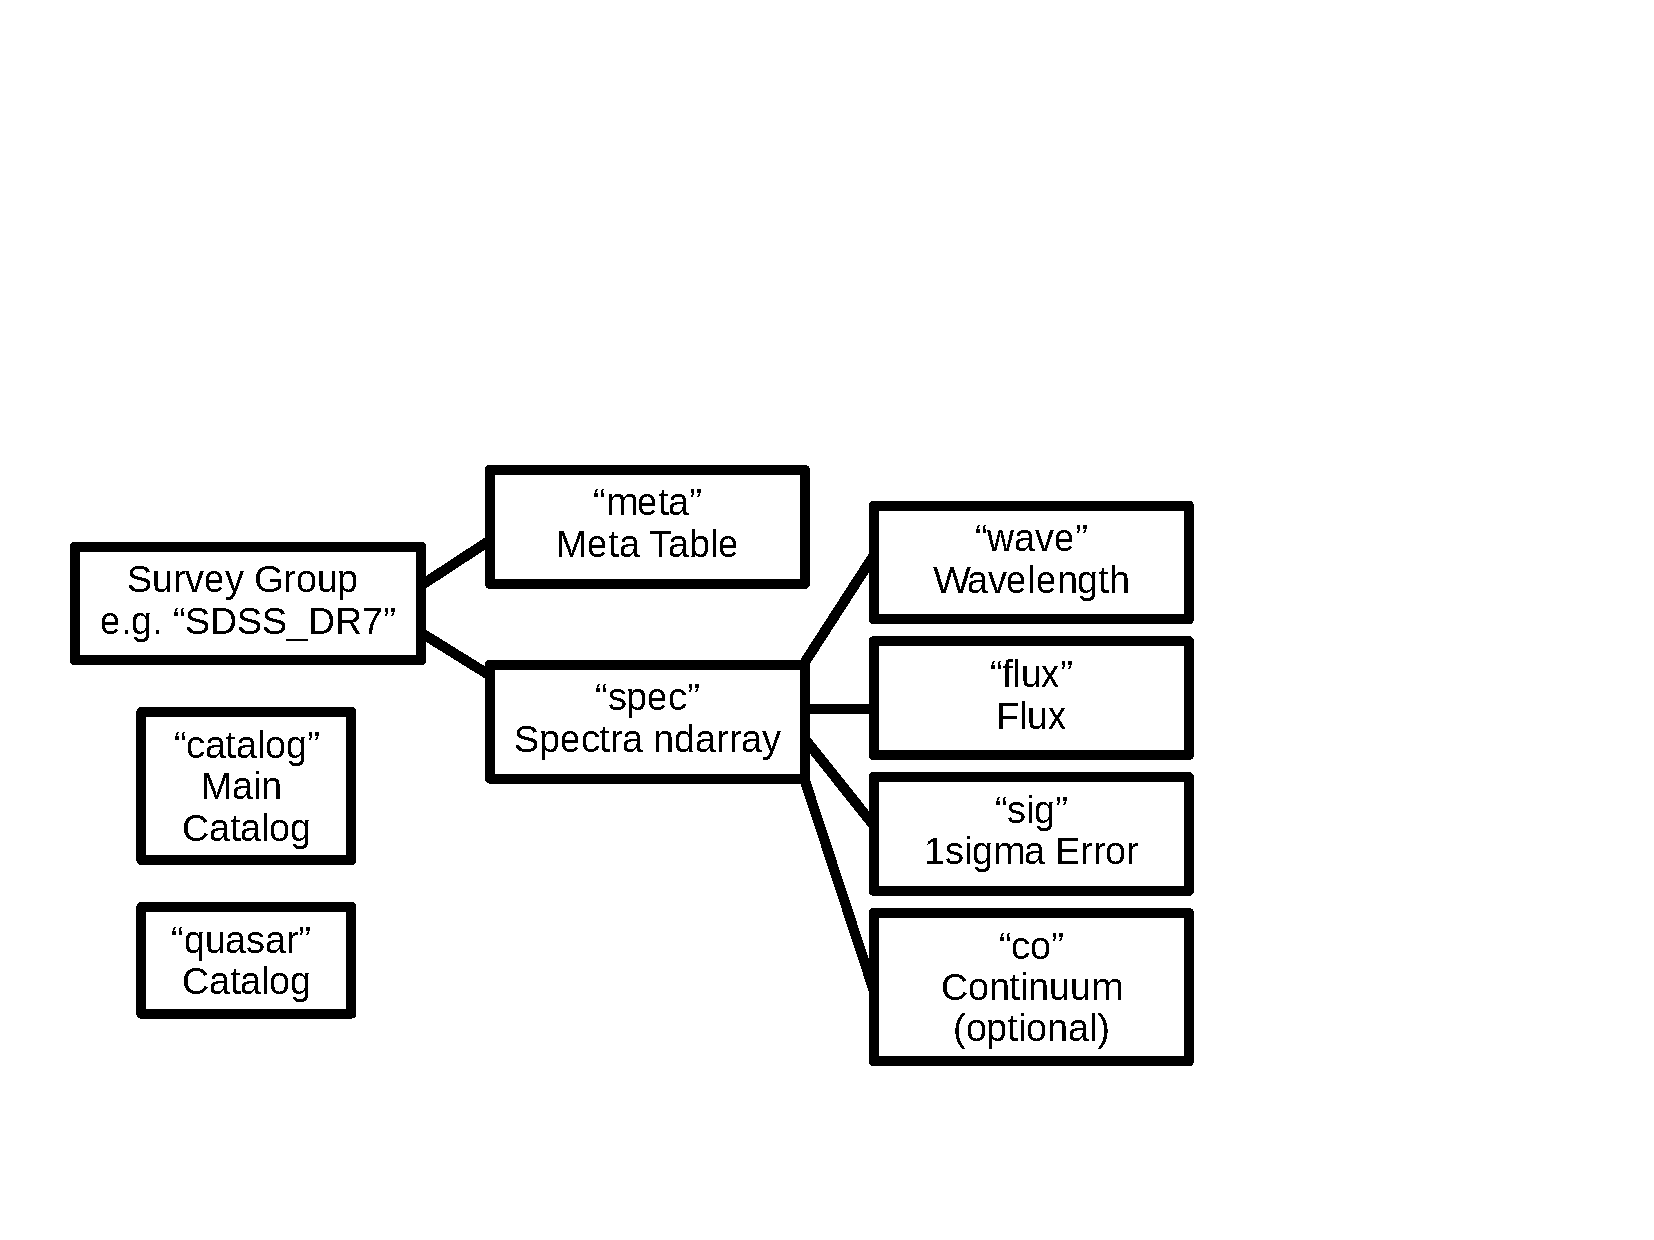
\includegraphics[width=6in]{architecture_v02.pdf}
\caption{Schematic describing the architecture of 
the {\it igmspec} database.
}
\label{fig:arch}
\end{figure}


\end{document}
